\documentclass[12pt,a4paper]{article}
\usepackage[UTF8]{ctex} % 支持中文
\usepackage{geometry}
\usepackage{graphicx}
\usepackage{amsmath}
\usepackage{float}
\usepackage{subfigure}
\usepackage{booktabs} % 表格美化
\usepackage{cite}
\usepackage{ulem}
\usepackage{array}
\usepackage{multirow}
\usepackage{hanging}


\newcolumntype{M}[1]{>{\centering\arraybackslash}m{#1}}
\newcommand{\down}[2]
{
	$\Delta_{\text{#1}}\approx{#2}$
}

% 设置页面边距
\geometry{left=2.5cm,right=2.5cm,top=2.5cm,bottom=2.5cm}

\title{\Huge{\textbf{\uuline{实\ 验\ 报\ 告}}}}
\author{\uline{少年班}\ 学院 \quad 姓名:\ \uline{顾泓宇} \quad 学号:\ \uline{PB23000078} \quad 实验日期:\ \uline{2024-5-27}}
\date{}

\begin{document}
	\maketitle
	
	\section{实验题目}
	用分光计测三棱镜折射率
	
	\section{实验目的}
	1.了解分光计的结构及工作原理，掌握分光计的调整方法和调节技巧。\\
	\hspace*{2em}2.用最小偏向角法测量玻璃三棱镜的折射率。\\
	\hspace*{2em}3.利用分光计探究三棱镜材料的色散。\\
	\hspace*{2em}4.探究分光计的应用技术和方法。
		
	\section{实验原理}
	\subsection{分光计的结构}
	分光计主要由底座、平行光管、望远镜、载物台和读数圆盘五部分组成，结构如图1所示。\\
	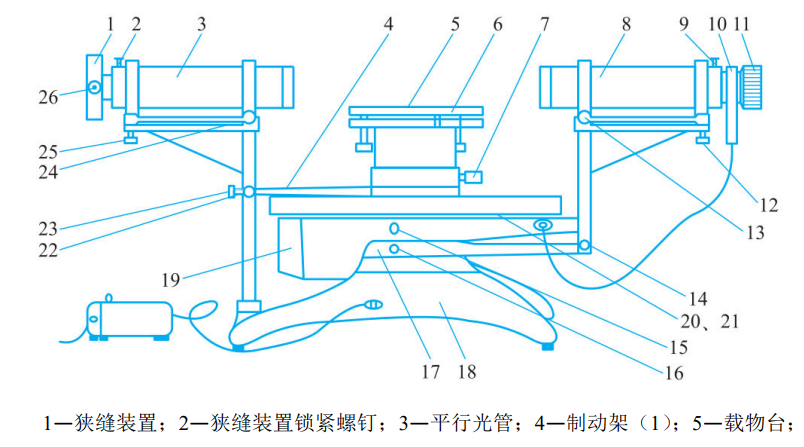
\includegraphics{1.png}\\
	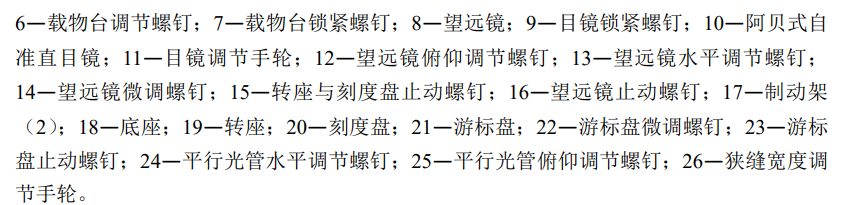
\includegraphics{2.png}
	
	\subsection{分光计的调整原理和方法}
	调整分光计，最后要达到下列要求：\\
	\hspace*{2em}1.望远镜对平行光聚焦.\\
	\hspace*{2em}2.望远镜光轴与仪器主轴垂直.\\
	\hspace*{2em}3.平行光管出射平行光.\\
	\hspace*{2em}4.平行光管光轴与仪器主轴垂直，与望远镜光轴共轴\\
	主要分为
	

	
	\section{参考文献}
	[1]. 单摆法测重力加速度. 实验讲义.2024
	
\end{document}